\section{Hardware Components} \label{HW}

A design goal for the PCAL upgrade of the FEC was an improvement in both light yield and spatial resolution within a more limited budget.  Compared to the early 1990s when the EC was designed, the lower price of wavelength shifting (WLS) fibers combined with new techniques for the production of high light yield extruded scintillator has enabled this cost savings.  Use of embedded WLS fibers bypasses the need for costly low attenuation scintillator (such as the BC-412 used in EC) while the readout simplification enables further improvement in light yield.

Several studies were performed \cite{2007002,2007007,2009018} to select the optimal combination of light readout components (scintillator, WLS fiber and photomultiplier) needed to maximize the light yield.  Based on the results of measurements and the available price estimates, we concluded that the best choice for the PCAL components were: Fermilab (FNAL) extruded scintillator, the KURARAY Y11 multiclad 1 mm diameter WLS fiber, and the HAMAMATSU R6095 PMT, selected to have quantum efficiency $>$ 16$\%$ at 500 nm. It should be noted that the performance and price of extruded scintillators from Amcrys-Plast/Kharkov (Ukraine), WLS fibers G91A from BICRON and the HAMAMATSU PMT R1450 (selected to have $>$ 18$\%$ quantum efficiency at 500 nm) were not far from the best choice set and generally met the requirements for PCAL. 

\begin{figure}[hbt]
\centering
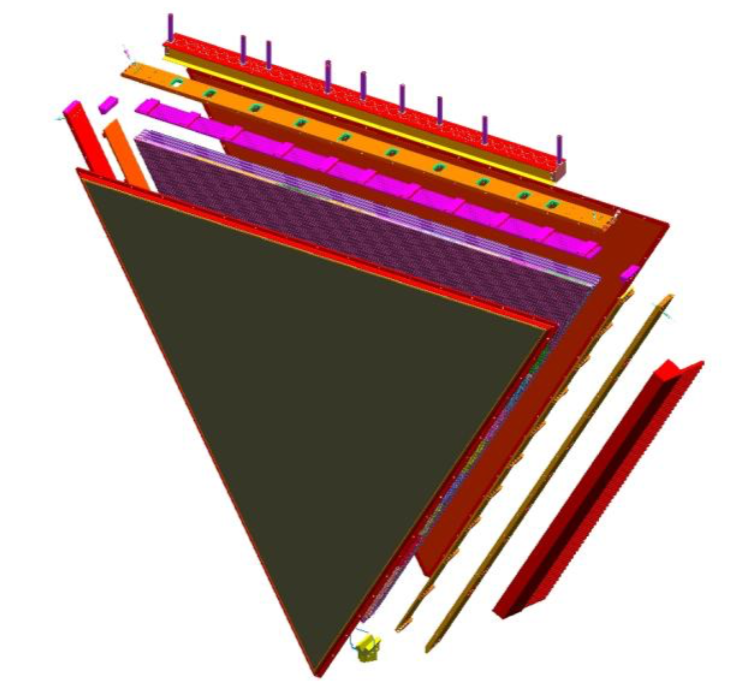
\includegraphics[width=0.95\columnwidth,keepaspectratio]{img/S4_0.png}
\caption{CAD model of the PCAL box showing the front/rear composite windows, sidewall supports and lead/scintillator sandwich.}
\label{fig:S4_0}
\end{figure}

\subsection{Mechanical Support}
The PCAL box consists of two composite windows of 25.4~mm ROHACELL structural foam core (FR-3715 Last-A-Foam, density 0.24~g~cm$^{-3}$) sandwiched between two 2 mm stainless steel sheets.  Each window set is held together by a stainless steel "L" frame welded around the perimeter.  The front and rear windows are bolted to three aluminum sidewalls which complete the structural members of the box (Fig.~\ref{fig:S4_0}).  All lead and scintillator layers inside the box are held in position by a retaining assembly attached to two of the sidewalls.  These retainers also create a space between the sidewall and the end of the scintillator strips.  This space together with machined slots and channels route the light readout fibers out of the box to the PMT housings (Fig. \ref{fig:S3_6}).  At the PMT readout end, the fibers pass through the three holes of the black PVC adapters to which the PMT will be mounted.  There the fibers are glued into the adapter, then milled, polished and coupled to the PMTs with optical grease (Fig. \ref{fig:S3_5}). The opposite ends of the fibers extend from the far end of the strips by $\sim 1$ mm and are spot glued to the scintillator.  

\begin{figure}[hbt]
\centering
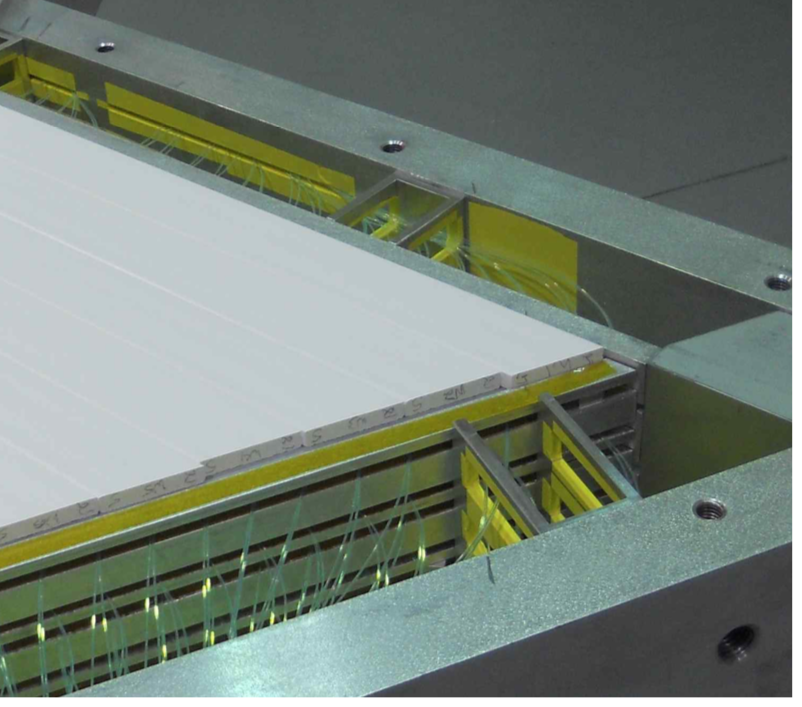
\includegraphics[width=0.95\columnwidth,keepaspectratio]{img/S3_6.png}
\caption[PCAL UVW Layers]{Retainer assembly at the corner of the VW and U readout sides of the PCAL box. Yellow mylar tape is applied at locations of potential abrasion of the WLS fibers.}
\label{fig:S3_6}
\end{figure}

\begin{figure}[hbt]
\centering
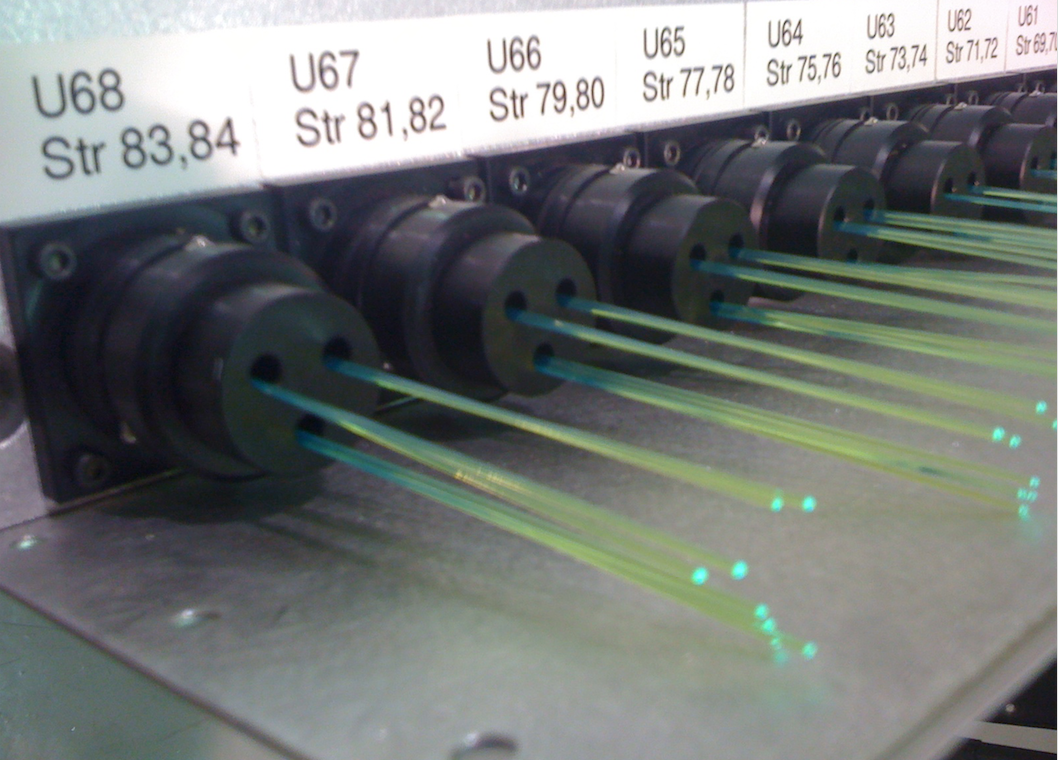
\includegraphics[width=0.9\columnwidth,keepaspectratio]{img/S3_5a.png}
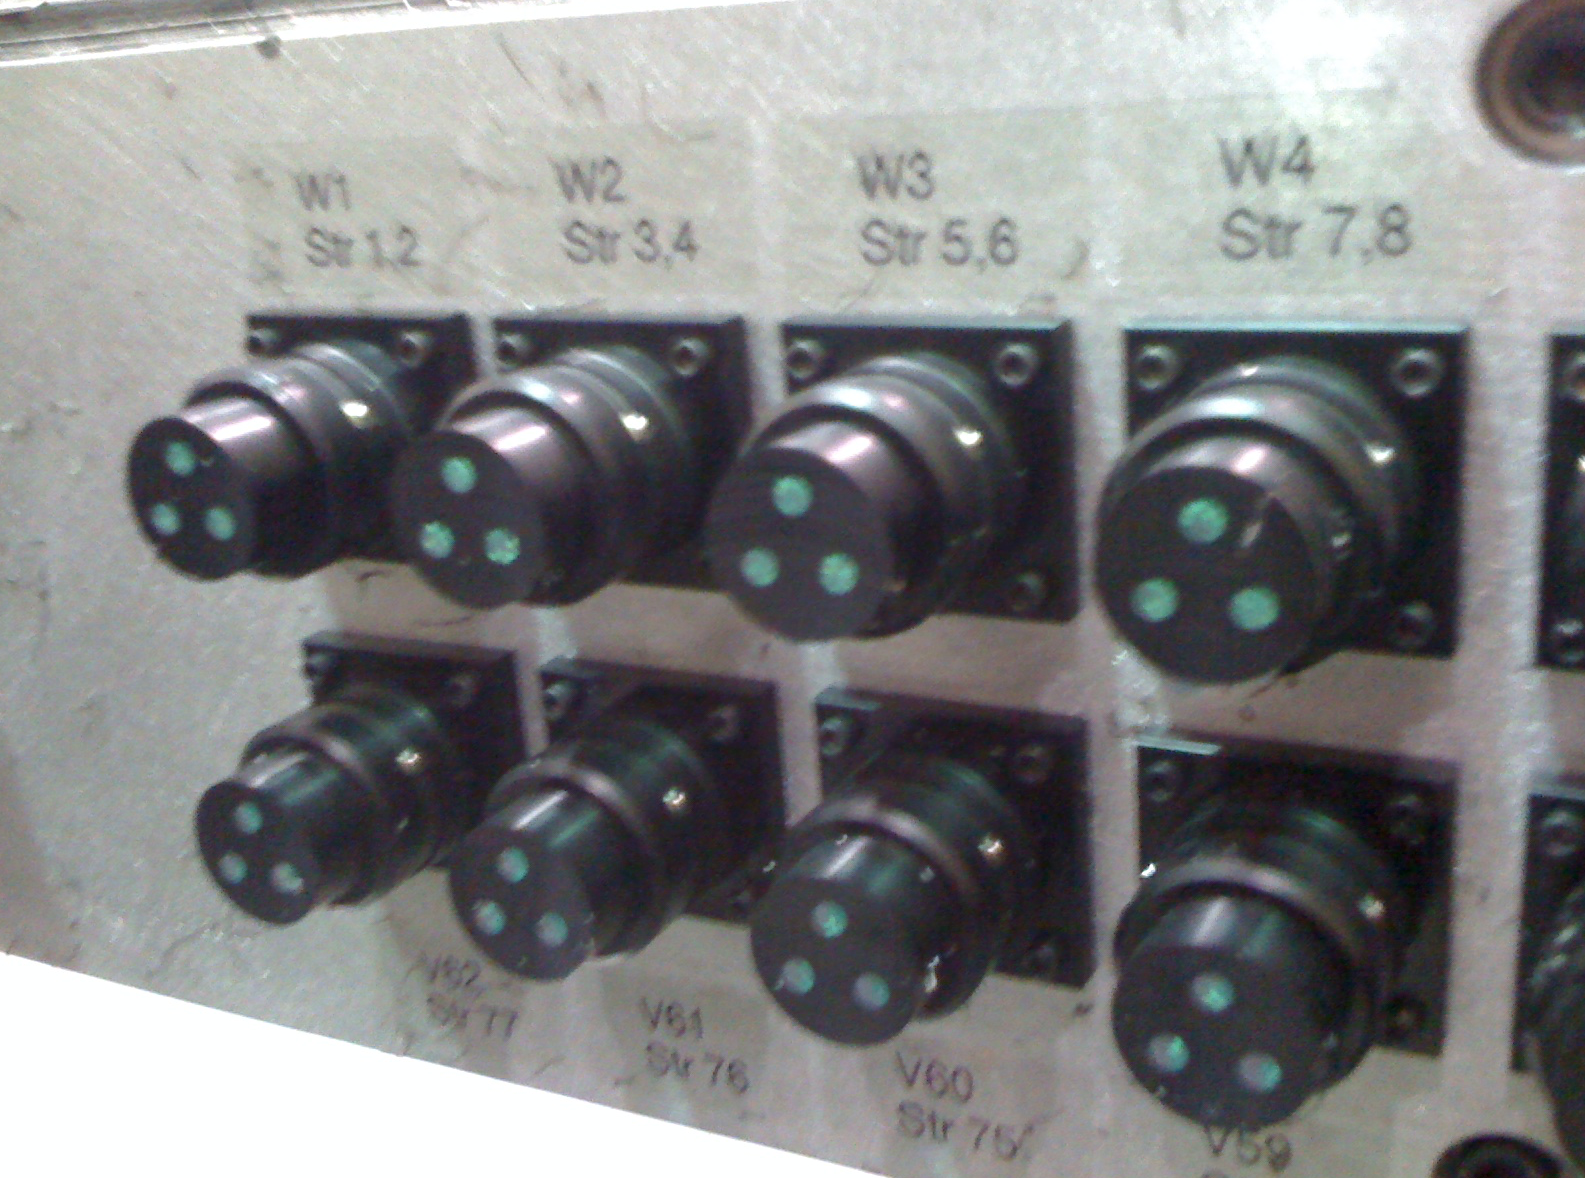
\includegraphics[width=0.9\columnwidth,keepaspectratio]{img/S3_5b.png}
\caption[PCAL UVW Layers]{Top: WLS fibers from scintillators extending from PMT attachment mounts fixed to the PCAL bulkhead. Bottom: WLS fibers after gluing, milling and polishing prior to PMT installation.}
\label{fig:S3_5}
\end{figure}

\subsection{Scintillators}

The scintillator strips used in PCAL were manufactured at the FNAL-NICADD Extrusion Line Facilty.  The nominal dimensions were 500 mm x 45 mm x 10 mm. The polystryene base of the scintillators was Dow STYRON 663 W. The primary dopant was 2,5-diphenyloxazole (PPO, 1$\%$ by weight). The secondary dopant was 1,4-bis (5-phenyloxazol- 2-yl) benzene (POPOP, 0.03$\%$ by weight).  A reflective surface coating of polystryene with 12$\%$ TiO2 of 0.25 mm nominal thickness was co-extruded during the manufacturing process.  Each strip has two holes through the length of the strip which were also co-extruded. The holes are intended to allow easy insertion of two 1 mm diameter fibers.

Scintillators from FNAL were delivered to JLAB with two lengths: 420 cm (1450 strips used for U-views) and 450 cm (2710 strips used for V,W-views).   Cutting of the strips was performed at JLAB and at the College of William and Mary (WM). The average width for scintillators to be used in a given layer was measured before the scintillators were cut, and the final cut length of the strips needed to fit within the triangular area was chosen based on this average to avoid buildup of errors during stacking.  The largest deviation from the design width of 45 mm was less than 0.3 mm, compared to the specified  tolerance for this dimension of $\pm$~1 mm.

\subsection{Wave Shifting Fibers}
Charged particles traversing the scintillator strips produce an emission spectrum ranging between 370-450 nm. The photons are down-converted and transported to the photomultipliers via the WLS fibers. An initial design for the fiber readout proposed using three WLS green fibers embedded in straight grooves running the length of the scintillator surface, and the R$\&$D studies discussed above \cite{2007007} were based on prototypes of this configuration.  A later study \cite{2009018} showed that through-holes inside the scintillator would enhance the light yield, since the fiber would be fully enclosed. The question arose as to how the holes can be efficiently filled with epoxy for the large scintillator pieces avoiding air bubbles and pockets. Also it was important to characterize the light tranmission characteristics of the scintillator with and without epoxy.

Finally it was concluded \cite{2010012} that while a gluing procedure could be developed with good reproducibility, careful and time consuming attention was required for large scale production.  These same studies also showed that two WLS fibers per hole without glue gives approximately the same transmission characteristics as a single fiber with glue (Fig. \ref{fig:S4_4}.  It was also found that less attenuation was produced without glued fibers. The added expense of extra fiber was more than offset by a much faster and simplier assembly procedure together with a likely more uniform light collection efficiency. 

\begin{figure}[hbt]
\centering
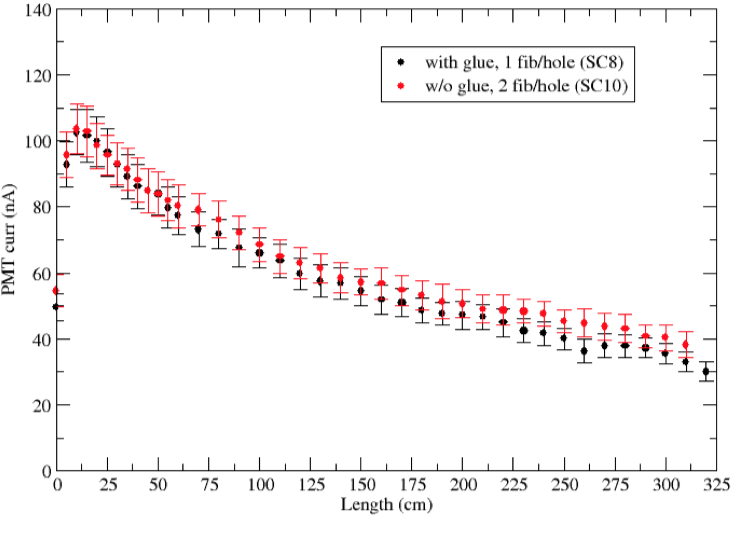
\includegraphics[width=0.85\columnwidth,keepaspectratio]{img/S4_4.png}
\caption{Relative light yield of various WLS readout fiber configurations.  Top and bottom plots compare different gluing procedures for fibers secured in holes filled with epoxy.}
\label{fig:S4_4}
\end{figure}

\subsection{Photomultiplier tubes}
Assembly and testing of all 1200 of the Hamamatsu R6095 PMTs assigned to PCAL was performed by students at James Madison University. Fig.~\ref{fig:S4_PMT} shows the individual elements of each PMT assembly. Each HV divider supplied with the PMT was tested for correct voltage at the pins.   Base assembly consisted of soldering HV, signal and ground cables between the divider and connector terminals on the end cap.  Spacers were cut and installed on either side of the spring to provide the desired compression force between the PMT and fiber adapter upon installation.  DC dark current measurements were made at 1000V for PMT acceptance testing and stored in a MYSQL database for later reference.  The  JMU dark current measurements showed a considerably small mean and variance compared to the test data from Hamamatsu as shown in Fig.~\ref{fig:S4_PMT_2}. 

\begin{figure}[hbt]
\centering
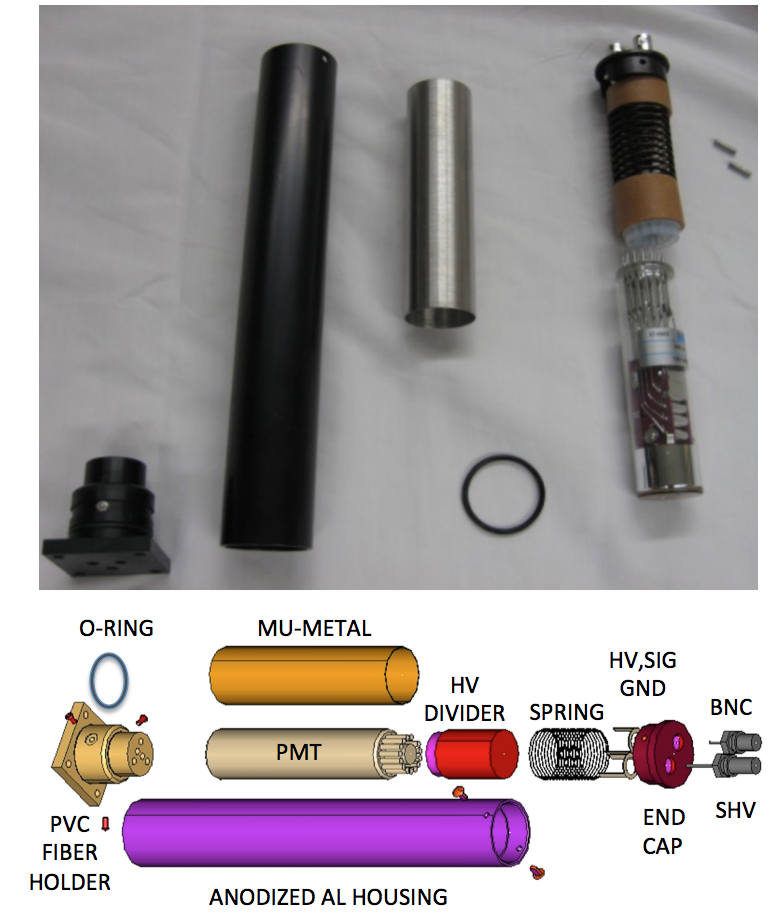
\includegraphics[width=0.85\columnwidth,keepaspectratio]{img/S4_PMT.png}
\caption{Photograph and schematic shows housing assembly for Hamamatsu R6095 1" diameter PMT used in PCAL.}
\label{fig:S4_PMT}
\end{figure}

\begin{figure}[hbt]
\centering
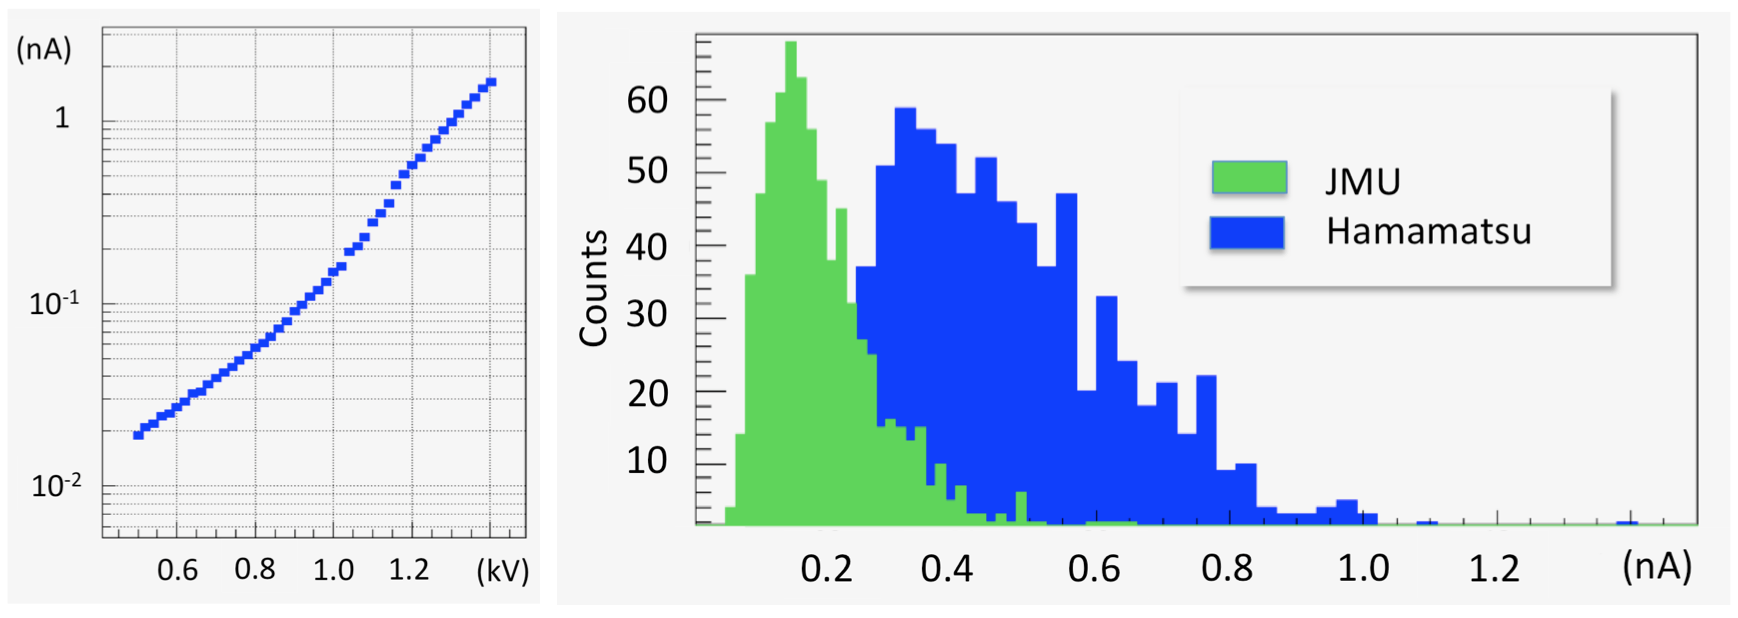
\includegraphics[width=1.0\columnwidth,keepaspectratio]{img/S4_PMT_2.png}
\caption{LEFT: Typical measurement of anode dark current vs voltage for Hamamatsu R6095 PMTs used in PCAL. Acceptance testing was performed at 1000 V.  RIGHT: Distribution of PMT anode dark current measurements from JMU and from Hamamatsu.  The JMU distribution mean is 0.2 nA.}
\label{fig:S4_PMT_2}
\end{figure}

\subsection{Lead}

Between two scintillator layers, there is one lead layer. For each PCAL module, there are a total of 14 lead layers. Each layer consists of two right-angle triangle shaped sheets, where the hypotenuse of each triangle is parallel to the V or W sidewall. Thickness uniformity of each layer was checked using a CHECK·LINE TI-25DL ultrasonic thickness gauge with 72 sample points measured per layer (36 for each half-layer).  A droplet of coupling liquid between the transducer and lead was used to  ensure reproducible sound transmission for each measurement.  Distributions of these sample points from all 14 layers in each module is shown in Fig. \ref{fig:S4_5}.

\begin{figure}[hbt]
\centering
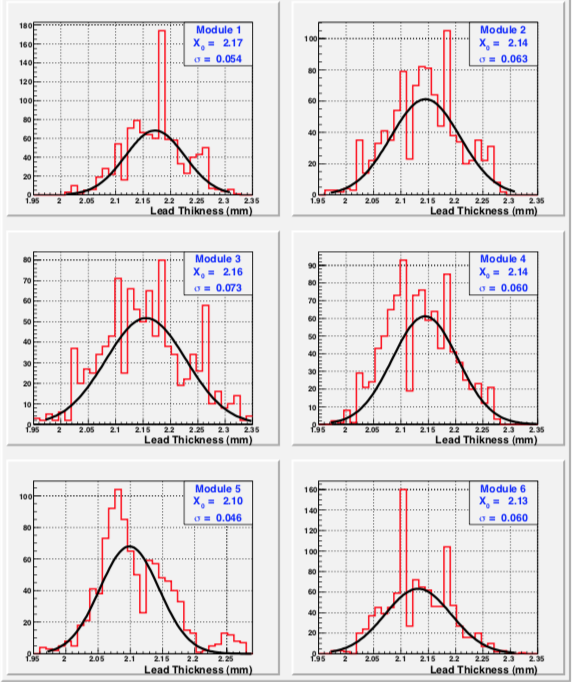
\includegraphics[width=0.95\columnwidth,keepaspectratio]{img/S4_5.png}
\caption{The distribution of measured thicknesses of the lead sheets for each PCAL module.}
\label{fig:S4_5}
\end{figure}


\section{Assembly and Installation}
Construction and acceptance testing of each PCAL module was performed at JLab.  Procedures included cleaning and assembly of the PCAL box, followed by stacking of the scintillator strips and lead sheets, routing of WLS fibers and spot gluing at both ends, milling and polishing of WLS fibers at the PMT readout adapter and ending with final shimming and installation of the downstream composite window.  Scintillator and fiber acceptance testing occurred in parallel in the same work area.


\subsection{Scintillator and fiber testing}
Prior to assembly of each PCAL module, acceptance testing of the transmission properties of both scintillator strips and WLS fibers was performed in a light-proof box using a computer automated system.  The apparatus used a PMT to measure the light output of the scintillator-fiber combination in response to a $^{90}$Sr beta source that was moved along the length of the scintillator strip. During scintillator testing, a set of four test fibers, glued to a plastic adapter in contact with the PMT photocathode, were inserted into the scintillator (two fibers per hole).  The PMT anode current was measured using a Keithley multimeter with 500 samples taken at 10 cm intervals along the strip.  Quality acceptance was based on uniformity of response and a typical exponential dependence on source position. Measurements were made for all of the longest ($>$200 cm) scintillator strips used in PCAL.

Studies at fixed distances of $x=10$~cm and $x=170$~cm showed light yield variations $<5\%$, while transverse variations at $x=10$~cm for four different source position were also $<5\%$, indicating good uniformity of the scintillator batch and no strong transverse dependence of fiber light collection efficiency.  More complete measurements of the light yield of the shortest and longest strips tested are shown in Fig.~\ref{fig:S5_0} where the position dependence $I(x)$ of the PMT current is shown fitted to a double exponential,

\begin{equation}
I(x) = A_S \exp(-x/\lambda_S)+A_L \exp(-x/\lambda_L)
\end{equation}

By fixing the short and long attenuation factors at their nominal values of $\lambda_S=70$~cm and $\lambda_L=400$~cm and refitting, it was found that the stability of the fitted amplitudes was around $17\%$ for $A_S$ and $5\%$ for $A_L$ for the group of scintillators studied. 

\begin{figure}[hbt]
\centering
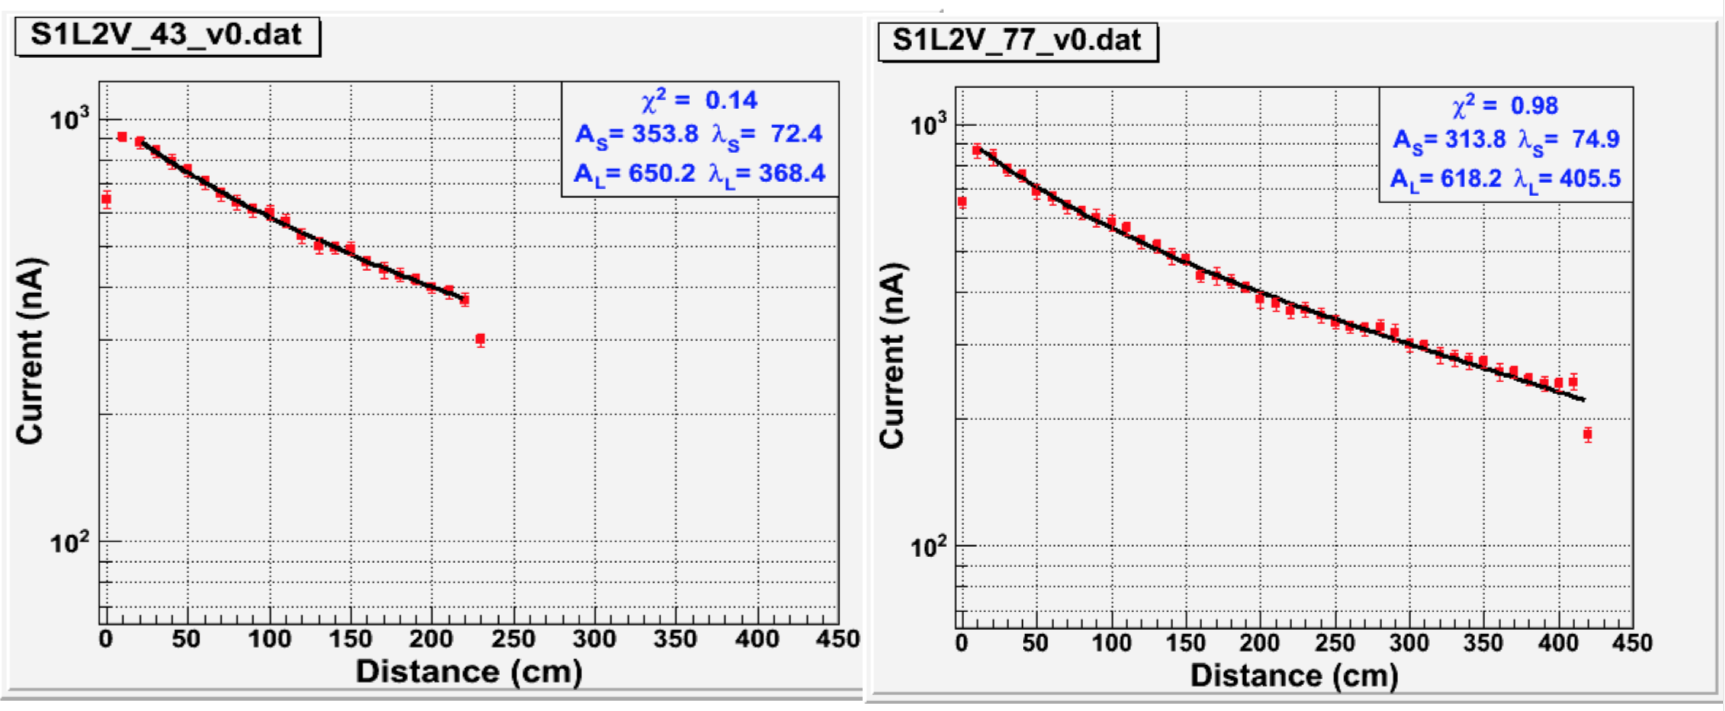
\includegraphics[width=0.95\columnwidth,keepaspectratio]{img/S5_0.png}
\caption{Measurements of PMT anode current versus $^{90}$Sr source position for PCAL scintillator fitted with 4 WLS readout test fibers. Here a double exponential is fitted to the shortest (LEFT) and longest (RIGHT) strips studied. }
\label{fig:S5_0}
\end{figure}

Testing of the WLS readout fibers was performed with the same apparatus, using a test scintillator 30 cm in length.  Five sets of four fibers each were selected at random for testing from each packaged bundle of 100.  A single measurement of the PMT current with and without fibers inserted was made at the midpoint of the scintillator.  In all cases fibers whose response was below the nominal measurement by $>15\%$ were found to have mechanical damage, although other fibers from the package were tested to double-check batch uniformity. Overall light yield stability of the fiber response was better than $7\%$.
 
\subsection{Lead-scintillator stacking}
Each PCAL box were cleaned with isopropanol to remove grease and debris from machining.  The bottom window was placed on a support table and side walls and retainers installed. Prior to scintillator stacking a 50$\mu$ Teflon sheet was laid down, followed by placement of the first U layer of 84 scintillator strips, beginning with the longest strip.  Gaps between scintillators were minimized both during placement and after each layer was complete using shimmed triangle pieces in the corners to push strips together.  Strips were also tightly bound between the retainers at the fiber readout end and flat spring clips at the opposite end to accomodate thermal expansion.

\begin{figure}[hbt]
\centering
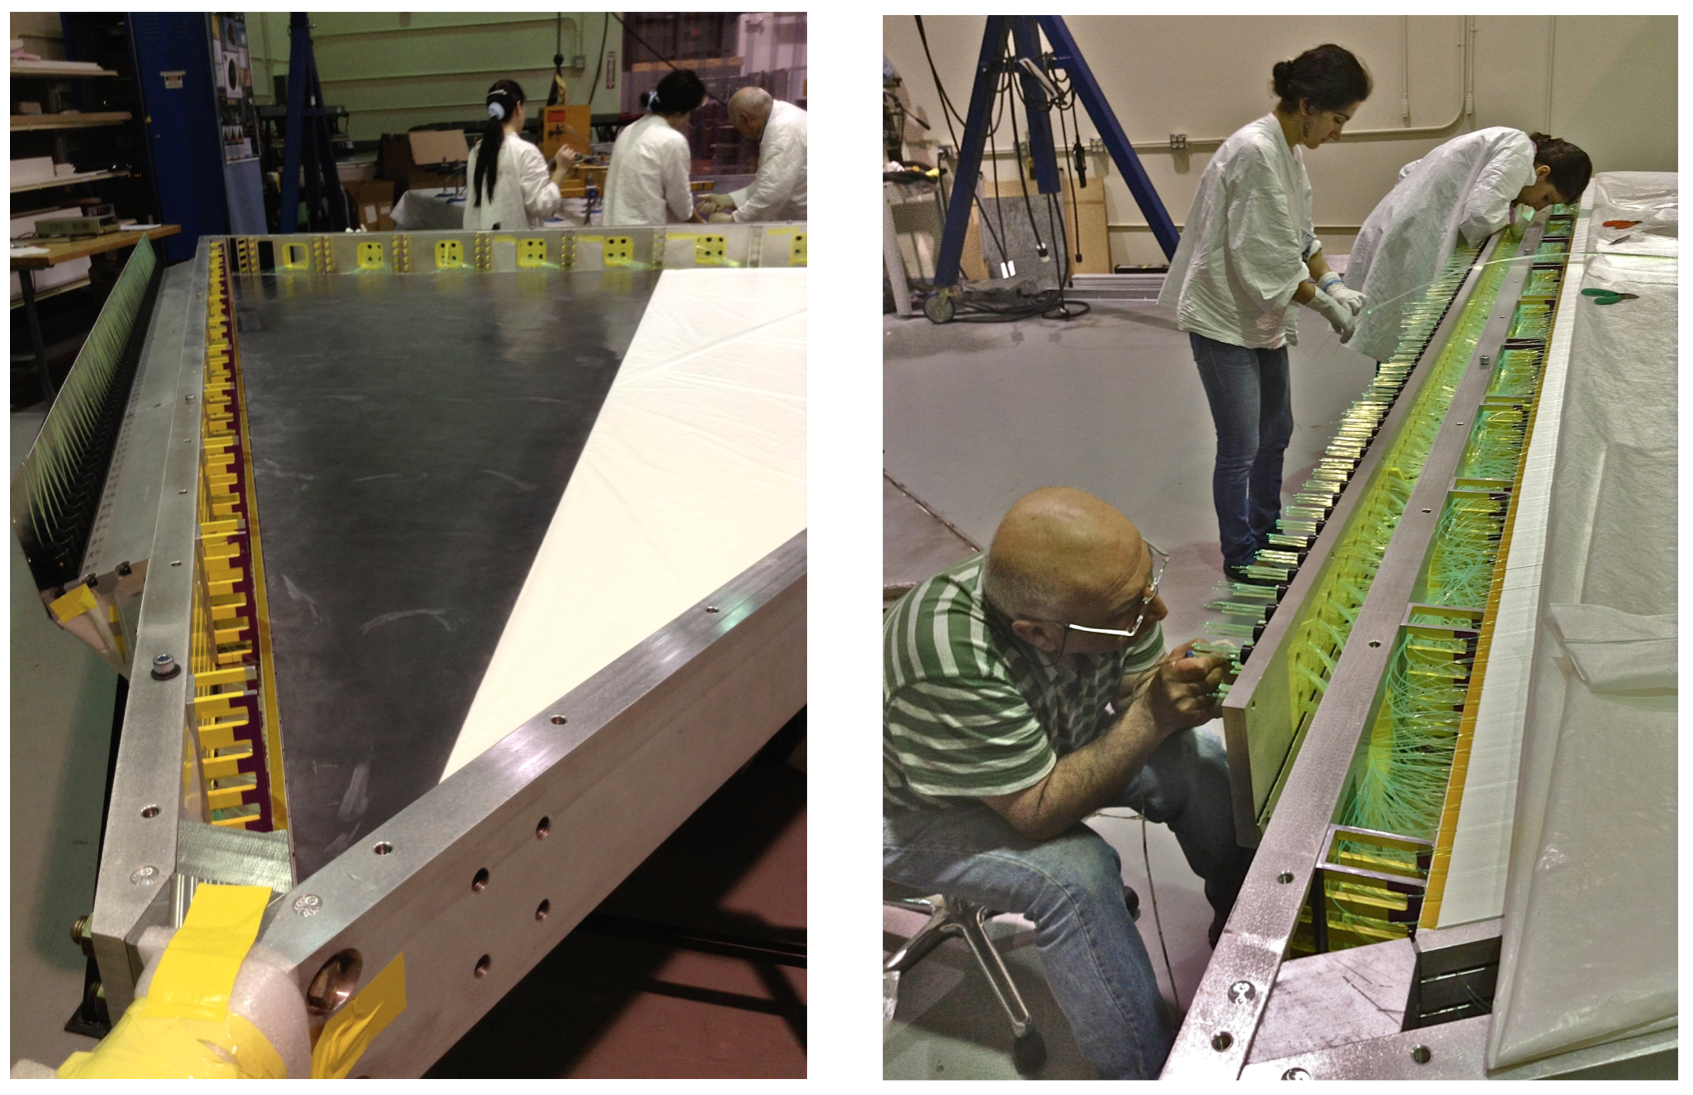
\includegraphics[width=0.95\columnwidth,keepaspectratio]{img/S5_2.png}
\caption{LEFT: Interior of PCAL box during scintillator/lead stacking.  Half layer of lead shown in place. RIGHT: WLS fiber routing and gluing operations.}
\label{fig:S5_2}
\end{figure}

Once all the scintillator strips were in place for a given layer, four WLS readout fibers were inserted one at a time into the two holes for each strip.  After scintillator insertion each fiber was cut to a length which was predetermined to allow the fiber to reach the PMT adapter holes and extend beyond by about 3 cm. (Fig.~\ref{fig:S5_2}).  This customized length was also designed to prevent sharp turns which fall below the minimum bend radius for these fibers for the particular routing needed.  After fiber installation and routing for all scintillators in the layer was complete, continuity and correct placement of each fiber was checked using a blue LED at the far end of ths trip and a photometer at the PMT base.  The final step was to spot glue all fibers at the far end to the scintillator.  This was done using DYMAX optical UV curing adhesive OP-4-20632.  Care was taken to leave an air hole to permit the flowing of dry nitrogen through the PCAL volume during its lifetime. 

Lead sheets were stored on a pallet and positioned into the PCAL box using a movable gantry and a crane with fine position control.  Suspended from the crane was a strongback with 12 vacuum pumped suction cups to uniformly lift the sheet and place it precisely in position, making sure the edge of the scintillator matched the edge of the lead plate.  Each lead layer was divided into two half-sheets to make installation more manageable.  For each PCAL module a total of 14 lead sheets and 15 scintillator/WLS layers were installed.

\begin{figure}[hbt]
\centering
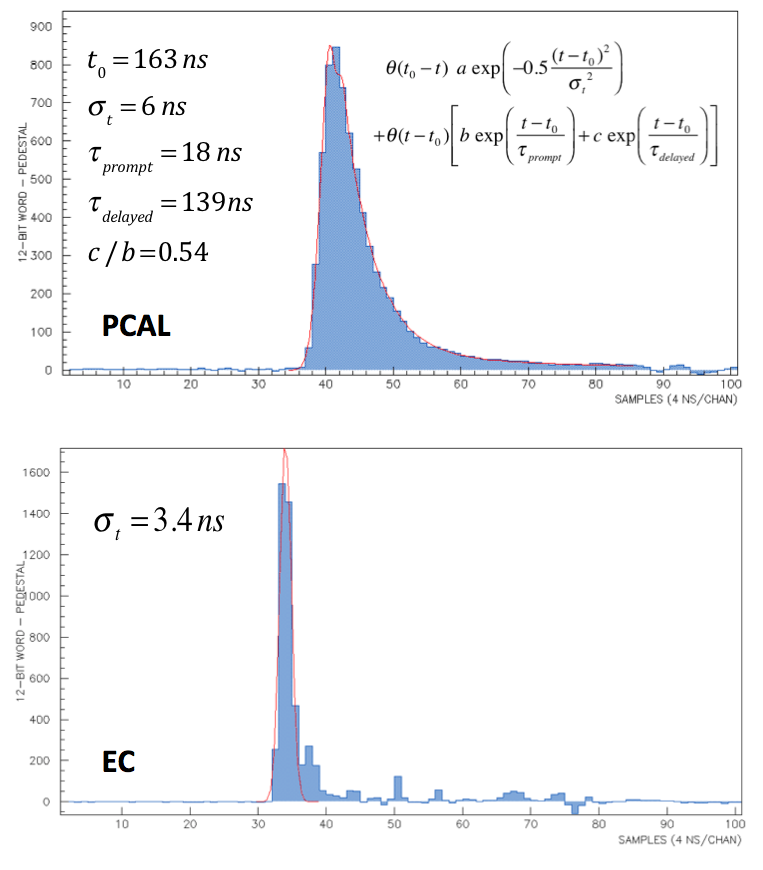
\includegraphics[width=0.95\columnwidth,keepaspectratio]{img/S5_3.png}
\caption{Comparison of pedestal subtracted fADC waveforms for PMTs in PCAL (top) and EC (bottom) PMTs.  Energy deposition resulted from cosmic triggers, where larger than typical amplitudes were selected to illustrate waveform shape. Fits to the PCAL shape used the expression shown, with typical fit parameters indicating the prompt and delayed components.   }
\label{fig:S5_3}
\end{figure}

\subsection{Cosmic Tests} \label{CRT}
Initial evaluation of PCAL performance was performed immediately after construction of each module using a test DAQ setup adjacent to the assembly area.  PMT installation and cabling was followed by gradual application of HV and the use of raw discriminator scaler data to identify and repair malfunctioning PMTs and sources of excessive noise.  Repairs were dominated by breakdown noise requiring extra mylar film insulation, cold solder joints of ground braids within the HV dividers, and pinhole light leaks in the RTV beads used to seal external sheet metal housings. 

Test procedures included using cosmic muon data to establish digitization parameters for the fADCs based on measurement of the PMT pulse waveforms and to perform initial PMT gain matching.  Fig.~\ref{fig:S5_3} (top) shows an example PCAL waveform for a 100 sample window aperture, where each sample is 4 ns.  Location of the pulse within the window was offset to reserve the first 15-30 samples for mean pedestal measurements needed to provide a baseline for setting the readout threshold.  Thresholds were set at 20 counts above the mean pedestal for calibration runs, and at about 70 counts for production runs at high luminosity.  All calibration and production fADC data were taken without compression or firmware integation to enable offline analysis for optimization of pulse integration, timing and background suppression for initial CLAS12 data taking.

Compared to the EC PMT waveform shown at the bottom of Fig.~\ref{fig:S5_3}, which has a very short duration and risetime of 2-3 ns, the PCAL waveform leading edge has a 6 ns rise and a subtantially extended duration, with both prompt and delayed components.  The PCAL prompt response is likely due to the convolution of both the slower polystyrene ($t_{1/2}=2-3$~ns) and Kuraray Y11 fiber ($t_{1/2}=7-12$~ns) response times compared to the much faster BC-412 ($t_{1/2}=1$~ns) scintillator used in EC.  Due to the delayed response about 35 samples above threshold were necessary to capture 97$\%$ of the integrated PCAL waveform.  

The next step was to obtain an initial set of HV settings which gain matched the PMTs.  After a short period of PMT stabilization, each assembled module was calibrated using a loose cosmic trigger requiring hits in 2 out of 3 of the U,V,W views.  The 1.2 kHz trigger rate was reduced by a factor of 20 using a software multiplicity cut to select near vertical muons before writing data to disk.  This ensured a uniform minimum ionizing energy deposition of 10 MeV for the five scintillators viewed by each of the U,V,W PMTs. Events were selected close to the readout end to minimize light attenuation and PMT HV settings were adjusted to normalize all MIP Landau distributions to the same ADC channel (Fig.~\ref{fig:S5_4} using a power law relation between voltage and the desired relative gain change $\Delta V/V = (\Delta G/G)^{1/n}$.  The value of the exponent $n$ needed to obtain rapid convergence was obtained with a few trial runs.  Overall gain matching at the level of 3-5$\%$ was achieved.

These preliminary studies provided the starting point for more extensive calibrations in Hall B described in Section \ref{Calibration}.  Also information on gain stability over the substantial storage time of some PCAL modules between contruction and installation in Hall B was desirable, as well as on any systematic differences in the response to muons with PCAL in a horizontal test position compared to the vertical position on the Forward Carriage.  Finally studies of long term changes in light attenuation of the WLS fibers in PCAL will include these first measurements.

\begin{figure}[hbt]
\centering
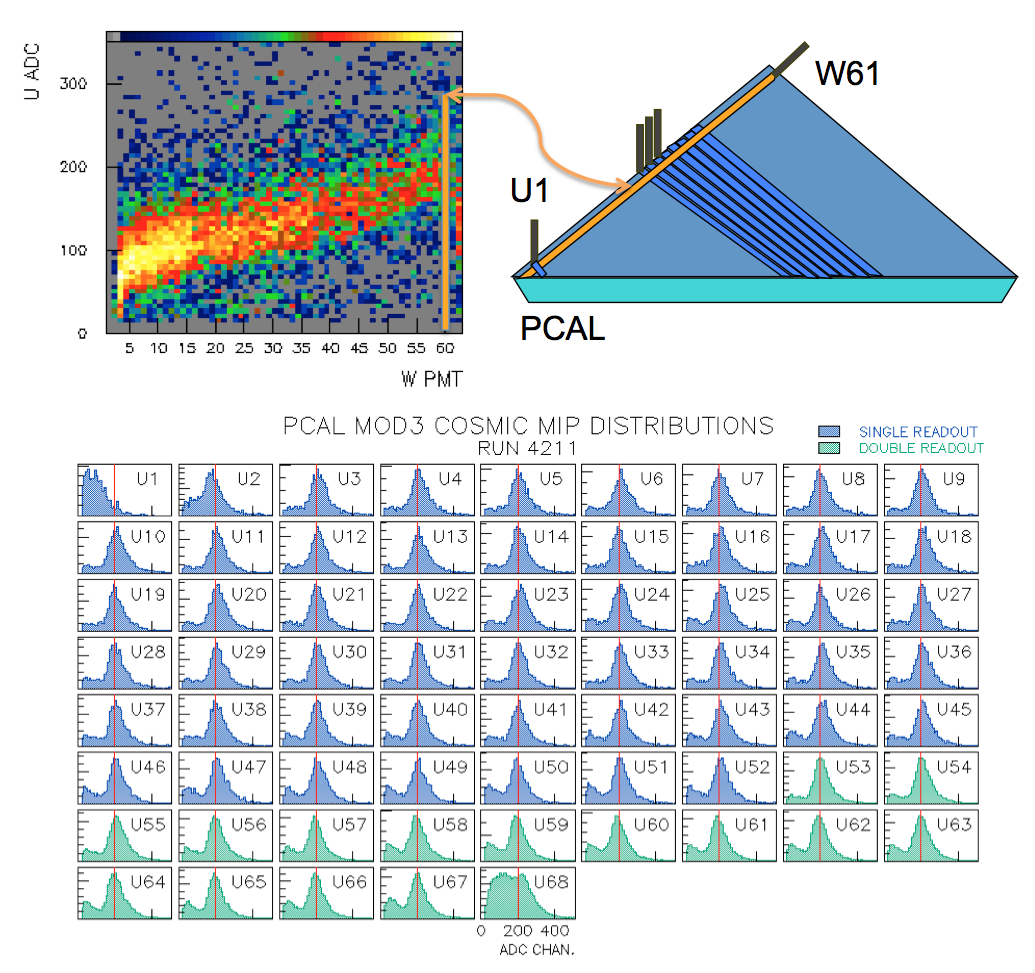
\includegraphics[width=0.95\columnwidth,keepaspectratio]{img/S5_4.png}
\caption{TOP: Schematic shows method used to perform PMT gain matching.  The U strip PMTs use crossing W strips as a proxy for light readout distance, while a multiplicity cut $N_u=N_v=N_w=1$ vetos non-vertical muons.   The left plot shows the attenuation of readout light in a U PMT from cosmic hits when plotted versus W PMT strip number.  All U PMT gains are adjusted to center the Minimum Ionizing Particle (MIP) ADC peak at channel 200, using W strip 61 to fix the readout distance at minimum attenuation.  BOTTOM: Summary of MIP calibration for all U strips.  Edge strips U1 and U68 show contributions from non-vertical muon trajectories which cannot be vetoed.}
\label{fig:S5_4}
\end{figure}

\subsection{Installation in Hall B}
Each PCAL module was mounted on the forward carriage (FC) directly in front of the existing EC module, using an installation tool suspended from the overhead crane consisting of a strongback and a counterweight to offset the 8 ton PCAL weight (Fig.~\ref{fig:S5_1}).  The PCAL nose was bolted to a central hub on the FC apex, while brackets on the V and W corners mounted to arms welded to the FC.   

\begin{figure}[hbt]
\centering
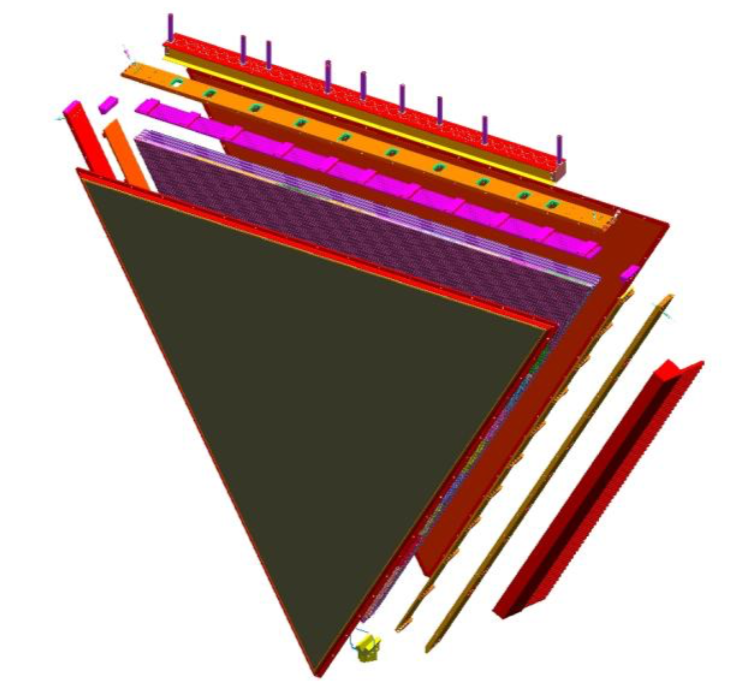
\includegraphics[width=0.95\columnwidth,keepaspectratio]{img/S5_1.png}
\caption{LEFT: Installation of PCAL module onto the forward carriage in Hall B at the Sector 5 position. U PMTs fit into the gap between the EC modules. RIGHT: PCAL module installed in front of the existing Sector 5 EC module. Yellow lifting fixtures were later removed. }
\label{fig:S5_1}
\end{figure}

The FC VME/VMX crates and HV mainframes are installed in six groups of racks on three levels which are located behind each of six sectors containing the PCAL/EC/FTOF/LTCC modules (and RICH in sector 4). The calorimeters use both CAEN 1527LC and 4527 HV supplies
outfitted with negative polarity 24-channel A1535N cards which fit into slots at the rear of each mainframe. The PCAL HV cards are housed in the same mainframe used by FTOF.  

Output signals from PCAL PMTs are routed to the FC with a single run of RG-58 coaxial cable. The EC PMT signals use RG-8 cable with RG-58 patch cables at both ends for a more flexible routing geometry.  Both EC and PCAL rely on passive resistive splitters designed and built at the University of Virginia to distribute signals to the TDC and ADC VME/VXS crates.  The split ratio is 2:1 for PCAL and 3:1 for EC.  For both calorimeters the larger signal goes to the ADC modules.  Mapping of patch cables from the splitter to electronics follows the same detector mapping used for the input to the splitters.

From the splitter, thin coax patch cables are routed to JLab DSC2 leading edge discriminators for pulse timing measurements and JLab 250~MHz 12-bit flash ADCs (fADC250) for pulse amplitude measurements.  Ribbon cables connect the DSC2 with CAEN 1190A TDCs which have 100~ps LSB resolution. The fADC250 and DSC2/TDC modules are housed in separate VXS crates.  The fADC250/VXS crate contains the JLab VXS Trigger Processor (VTP) in a special switched slot which is used to process energy and hit data for trigger decision making.

All 2304 HV and RG-58 signal cables were manufactured by students at Ohio University.  The thin coax interconnection cables were  manufactured by students at Norfolk State University.  Both groups also particpated in cable installation in the test setup and on the forward carriage in Hall B.  





